\documentclass[conference]{IEEEtran}

% ========= 日本語対応(LuaLaTeX推奨) =========
\usepackage{luatexja}
\usepackage{luatexja-fontspec}
\setmainjfont{HaranoAjiMincho}
\setsansjfont{HaranoAjiGothic}

% ========= 一般パッケージ =========
\usepackage{amsmath,amssymb}
\usepackage{graphicx}
\usepackage{booktabs}
\usepackage{array}
\usepackage{url}
\usepackage[hidelinks]{hyperref}
\usepackage{cite}

% ========= 図・グラフ =========
\usepackage{tikz}
\usetikzlibrary{arrows.meta,decorations.pathreplacing,calc,patterns}
\usepackage{pgfplots}
\pgfplotsset{compat=1.17}

% ========= タイトル =========
\title{DRAM技術導入とその戦略的位置づけ(1997--2001)\\
\large 酒田FabにおけるDRAM/PSRAMとロジック展開の関連}

% ========= 著者情報 =========
\author{%
  \IEEEauthorblockN{三溝 真一 (Shinichi Samizo)}%
  \IEEEauthorblockA{独立系半導体研究者(元セイコーエプソン)\\%
  Independent Semiconductor Researcher (ex-Seiko Epson)\\%
  Email: \href{mailto:shin3t72@gmail.com}{shin3t72@gmail.com}\\%
  GitHub: \url{https://github.com/Samizo-AITL}}%
}

\begin{document}
\maketitle

\begin{abstract}
\textbf{(日本語)}\\
本論文は,1997年から2001年にかけてセイコーエプソン酒田事業所が
三菱電機からの技術移管を通じて \mbox{0.5\,$\mu$m} $\rightarrow$ \mbox{0.35\,$\mu$m} $\rightarrow$ \mbox{0.25\,$\mu$m} の
DRAMプロセスを短期間で習得し,得られたプロセス知見を
先端ロジック,高耐圧混載CMOSへ展開して液晶ドライバー製品化に結びつけた
技術的・戦略的過程を,筆者の実体験に基づき整理する。
主要な不良モード(Pause/Disturb Refresh)の物理起源と対策,
および量産歩留まりの推移を示し,獲得した知見がその後の
事業ドメインへどのように接続されたかを考察する。\\[1ex]

\textbf{(English)}\\
This paper reviews 1997–2001, when Seiko Epson’s Sakata Fab
assimilated DRAM processes (0.5\,$\mu$m → 0.35\,$\mu$m → 0.25\,$\mu$m) transferred from Mitsubishi Electric.
The acquired know-how was extended beyond DRAM to advanced logic
and high-voltage mixed CMOS, leading to LCD driver products.
Key failure modes (Pause/Disturb Refresh), countermeasures, and yield evolution
are summarized based on the author’s on-site experience.
\end{abstract}

\begin{IEEEkeywords}
DRAM, VSRAM/PSRAM, 0.25\,$\mu$m process, retention failure, disturb failure, Sakata Fab, technology transfer, high-voltage mixed CMOS, LCD driver, process learning;
(日本語)DRAM,VSRAM/PSRAM,0.25\,$\mu$mプロセス,リテンション不良,ディスターブ不良,酒田Fab,技術移管,高耐圧混載CMOS,液晶ドライバー,プロセス習得
\end{IEEEkeywords}

% =========================
\section{序論}
1997年,当時の半導体産業は \textit{Windows~95} の世界的普及や
Intel Pentium~II の登場を契機として急成長局面にあった。
製造技術面では,8インチウェーハラインと 0.35\,$\mu$m 世代プロセスの
量産化が進展し,DRAM およびロジックLSIの分野で国際競争が一層激化していた。

セイコーエプソンは,山形県酒田市に建設した 8インチFab
(酒田事業所)において,三菱電機からの技術移管を通じて
0.5\,$\mu$m $\rightarrow$ 0.35\,$\mu$m $\rightarrow$ 0.25\,$\mu$m
の三世代DRAMプロセスを短期間で習得した。
ただし狙いはDRAM事業の恒常化ではなく,
DRAMを媒体として最新プロセスを自前化し,
最終的にロジック/高耐圧混載CMOSや液晶ドライバーへ展開する点にあった。

本研究は,この「DRAM導入を目的ではなく手段とする」戦略的枠組みを,
筆者の現場経験に基づき実証的に整理するものである。
特に,立ち上げ初期の不良モード解析(Pause/Disturb Refresh Fail)と対策,
歩留まり改善プロセス,さらに獲得知見のロジック展開への接続を論じる。

% =========================
\section{第1章:0.5\,\texorpdfstring{$\mu$m}{μm} と 0.35\,\texorpdfstring{$\mu$m}{μm} 世代の立ち上げ}

\subsection{0.5\,$\mu$m 16M DRAM}
酒田Fabの最初の量産製品は0.5\,$\mu$m世代16M DRAM。
熊本Fabで実績のあるプロセスを移管し,設備親和性も高く,
短期間で安定量産に到達した。

\subsection{0.35\,$\mu$m 64M DRAM:洗浄フロー差異と「鏡写し」}
\textbf{初期の困難:}
1997年秋,試作30ロット超を投入したが形状不良が多発。
\textbf{原因究明:}
徹底調査の結果,熊本では「硫酸過水→アンモニア過水→塩酸過水」,
酒田では工程短縮で硫酸過水を省略—という\emph{洗浄フロー差}が主因。
\textbf{解決:}
フロー/装置条件/手順まで\emph{完全に鏡写し}移管することで解消し,
量産化に成功した。

\subsection{小括}
0.5\,$\mu$mは移管の忠実再現で早期安定,0.35\,$\mu$mは洗浄差が主因。
「一切の省略を許さない鏡写し」が次世代0.25\,$\mu$mの土台となった。

% =========================
\section{第2章:0.25\,\texorpdfstring{$\mu$m}{μm} 世代64M DRAMの立ち上げ}

\subsection{SCF方式と初期歩留まり}
三菱電機で確立済みの \emph{Short Cycle Feedback (SCF)} を継続採用。
短サイクルで評価\,$\leftrightarrow$\,フィードバックを回し,
本番初期歩留まり約65\%を達成。

\subsection{保持時間モデルと不良モード解析}
Pause Refresh 試験(32→64→128\,ms)で単ビット不良が散発・ランダム分布。
保持時間は
\begin{equation}
\tau = \frac{C_{\mathrm{cell}} \cdot V_{\mathrm{cell}}}{I_{\mathrm{leak}}}
\end{equation}
で与えられ,$I_{\mathrm{leak}}$ の増大が主因。
解析より\emph{拡散層ジャンクションリーク}に特定,フェイル座標の再現性から
\emph{プロセス条件起因の系統要因}と判断した(Fig.~\ref{fig:dram_cross_section}, Fig.~\ref{fig:failmap})。

\begin{figure}[t]
\centering
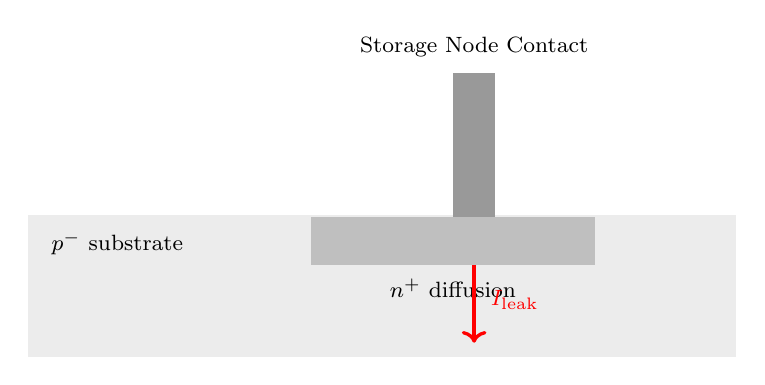
\begin{tikzpicture}[scale=1.8]
  \fill[gray!15] (-1,0) rectangle (4,-1.0); % p- substrate
  \node[anchor=north west] at (-0.9,-0.05) {\footnotesize $p^-$ substrate};
  \fill[gray!50] (1,-0.01) rectangle (3,-0.35); % n+ diffusion
  \node[anchor=north] at (2,-0.38) {\footnotesize $n^+$ diffusion};
  \fill[black!40] (2,-0.01) rectangle (2.3,1.0); % SN contact (filled box)
  \node[anchor=south] at (2.15,1.05) {\footnotesize Storage Node Contact};
  \draw[->,very thick,red] (2.15,-0.35) -- (2.15,-0.9);
  \node[anchor=west,red] at (2.2,-0.6) {\footnotesize $I_{\mathrm{leak}}$};
\end{tikzpicture}
\caption{DRAM セル断面の概念図。赤矢印は $n^+ \rightarrow p^-$ へのリーク $I_{\mathrm{leak}}$。}
\label{fig:dram_cross_section}
\end{figure}

\begin{figure}[t]
\centering
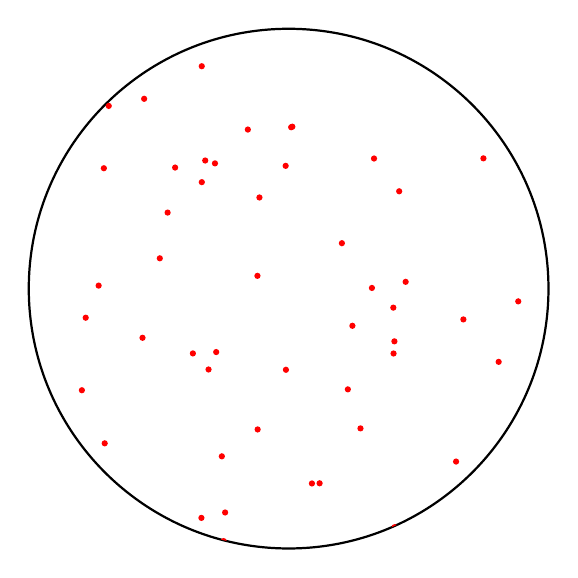
\begin{tikzpicture}[scale=0.22]
  \def\R{15}
  \draw[thick] (0,0) circle (\R);
  \begin{scope}
    \clip (0,0) circle (\R);
    \foreach \i in {1,...,60}{
      \pgfmathsetmacro{\xx}{(rnd*2-1)*\R}
      \pgfmathsetmacro{\yy}{(rnd*2-1)*\R}
      \fill[red] (\xx,\yy) circle (0.18);
    }
  \end{scope}
\end{tikzpicture}
\caption{Pause Refresh Fail のフェイルビットマップ例(ウエハ外周円+ランダム赤点)。}
\label{fig:failmap}
\end{figure}

\subsection{プラズマダメージ仮説}
ゲートエッチ後の酸化膜露出/LDDの繰返しアッシングで
酸素プラズマによる界面欠陥準位が生成しリーク増大—と推定。

\subsection{対策と効果}
\emph{O$_2$アッシング→硫酸剥離(ウエット)}に全面切替。
プラズマ曝露を根本排除し,Pause不良を大幅低減。
Table~\ref{tab:resist_flow} と Fig.~\ref{fig:yield_trend} にまとめる。

\begin{table}[t]
  \centering
  \caption{レジスト剥離フローの切替(Before/After)}
  \label{tab:resist_flow}
  \begin{tabular}{p{0.25\linewidth} p{0.65\linewidth}}
    \toprule
    従来(Before) & O$_2$アッシングによるドライ剥離 \\
    対策後(After) & 硫酸剥離によるウエット剥離 \\
    主効果 & プラズマ曝露ゼロ化,界面欠陥・ジャンクションリーク抑制 \\
    歩留まり & 65\% $\rightarrow$ 80\%台後半(Pause改善が支配) \\
    \bottomrule
  \end{tabular}
\end{table}

\begin{figure}[t]
\centering
\begin{tikzpicture}
\begin{axis}[
  width=\linewidth,height=6cm,
  ymin=0,ymax=100,
  ylabel={歩留まり(\%)},
  symbolic x coords={0.5\,\mu m,0.35\,\mu m,0.25\,\mu m,VSRAM},
  xtick=data,xticklabel style={align=center},
  xlabel={プロセス世代},
  grid=both,
  legend style={at={(0.5,-0.28)},anchor=north,draw=none,fill=none,font=\footnotesize},
  legend columns=2,clip=false
]
  \addplot+[semithick,mark=*]
    coordinates {(0.5\,\mu m,95) (0.35\,\mu m,20) (0.25\,\mu m,65) (VSRAM,30)};
  \addlegendentry{初期歩留まり}
  \addplot+[semithick,mark=square*]
    coordinates {(0.5\,\mu m,95) (0.35\,\mu m,86) (0.25\,\mu m,88) (VSRAM,80)};
  \addlegendentry{改善後}
\end{axis}
\end{tikzpicture}
\caption{酒田Fabにおける世代別歩留まり推移。}
\label{fig:yield_trend}
\end{figure}

\subsection{小括}
SCFで初期65\%,硫酸剥離への切替で80\%台後半へ。
「表面処理とプラズマ影響は軽視不可」という教訓を得た。

% =========================
\section{第3章:VSRAM(2001年)— Pause/Disturb対策と歩留まり改善}

\subsection{開発背景と初期状況}
モバイル向け低消費・90\,$^\circ$C保証が求められ,
0.25\,$\mu$m DRAM流用+内部リフレッシュで\emph{VSRAM}を実現。
しかし初期量産歩留まりは約30\%。

\subsection{顕在化した不良モード}
\begin{itemize}
  \item \textbf{Pause Refresh Fail}: リフレッシュ停止時に保持不足でデータ喪失。
  \item \textbf{Disturb Refresh Fail}: リフレッシュ中のWLが隣接セルを誤反転。
\end{itemize}

\subsection{物理的要因}
保持時間は $\tau=C_{\mathrm{cell}}V_{\mathrm{cell}}/I_{\mathrm{leak}}$。
温度上昇で $I_{\mathrm{junc}}$ は指数増加し(Fig.~\ref{fig:pause_temp_junc}),
バックバイアス強化で抑制可能。
一方,短チャネル化で $I_{\mathrm{off}}$ が増大(Fig.~\ref{fig:disturb_temp_sce})。

\begin{figure}[t]
\centering
\begin{tikzpicture}
\begin{axis}[
  width=\linewidth,height=6cm,
  xlabel={温度 [$^\circ$C]}, ylabel={ジャンクションリーク $I_{\mathrm{junc}}$(相対)},
  ymode=log, ymin=1e-2, ymax=1e2,
  xmin=25, xmax=100, xtick={25,40,60,80,90,100},
  grid=both, legend style={at={(0.5,-0.22)},anchor=north,draw=none,fill=none}, clip=false
]
  \addplot+[semithick,mark=*] coordinates {(25,0.02) (40,0.06) (60,0.3) (80,1.6) (90,3.2) (100,6.0)};
  \addlegendentry{$V_{bs}=-1$ V}
  \addplot+[semithick,mark=square*] coordinates {(25,0.01) (40,0.03) (60,0.12) (80,0.45) (90,0.9) (100,1.8)};
  \addlegendentry{$V_{bs}=-3$ V}
\end{axis}
\end{tikzpicture}
\caption{Pause:温度で $I_{\mathrm{junc}}$ が指数増大。バックバイアス強化で抑制。}
\label{fig:pause_temp_junc}
\end{figure}

\begin{figure}[t]
\centering
\begin{tikzpicture}
\begin{axis}[
  width=\linewidth,height=6cm,
  xlabel={温度 [$^\circ$C]}, ylabel={トランジスタリーク $I_{\mathrm{off}}$(相対)},
  ymode=log, ymin=1e-3, ymax=1e1,
  xmin=25, xmax=100, xtick={25,40,60,80,90,100},
  grid=both, legend style={at={(0.5,-0.22)},anchor=north,draw=none,fill=none}, clip=false
]
  \addplot+[semithick,mark=triangle*] coordinates {(25,0.004) (40,0.01) (60,0.05) (80,0.22) (90,0.45) (100,0.9)};
  \addlegendentry{CD=0.25\,$\mu$m}
  \addplot+[semithick,mark=*] coordinates {(25,0.01) (40,0.03) (60,0.15) (80,0.7) (90,1.4) (100,2.8)};
  \addlegendentry{CD=0.20\,$\mu$m}
\end{axis}
\end{tikzpicture}
\caption{Disturb:短チャネル効果で $I_{\mathrm{off}}$ 増大。温度上昇でも指数増。}
\label{fig:disturb_temp_sce}
\end{figure}

\subsection{対策と実装}
\textbf{Pause対策}—HF洗浄回数最小化(ゲート酸化膜残膜確保,SN近傍リーク低減),
バックバイアス強化($V_{bs}=-1\rightarrow-3$ V)。\\
\textbf{Disturb対策}—ゲートCD中心値の厳密管理,
バックバイアス強化,セルのチャネルドーピング若干増(動作範囲内,$V_\mathrm{th}$ 向上)。

\begin{table}[t]
\centering
\caption{Pause / Disturb 不良に対する主な対策}
\label{tab:counter}
\begin{tabular}{p{0.18\linewidth} p{0.28\linewidth} p{0.46\linewidth}}
\toprule
不良モード & 主因 & 主な対策 \\
\midrule
Pause   & ジャンクションリーク & HF洗浄制御,バックバイアス強化 \\
Disturb & 短チャネル効果       & CD管理,チャネルドーピング,バックバイアス強化 \\
\bottomrule
\end{tabular}
\end{table}

\subsection{効果と歩留まり推移}
Pause/Disturbは大幅低減。歩留まりは30\%→80\%台に回復し量産水準を達成。

\subsection{小括}
VSRAMの歩留まり改善知見は,直接ロジックへ展開はしないが,
以後の\emph{高耐圧混載CMOS}の設計余裕・工程設計の基礎データとなった。

% =========================
\section{第4章:0.18\,\texorpdfstring{$\mu$m}{μm} トレンチ系の評価と断念}

\subsection{背景}
NANYA 0.18\,$\mu$m(東芝系トレンチ)でVSRAM後継を検討。
高密度・低消費を狙うも,90\,$^\circ$C保証が厳しかった。

\subsection{課題の顕在化と結果}
Pause不足・Disturb増加・高温リークが顕著。
Fig.~\ref{fig:trench_area_leak} の通り,トレンチでは\emph{ジャンクション面積に比例}して
$I_{\mathrm{junc}}$ が増え,90\,$^\circ$Cで増加率がより大きい。

\begin{figure}[t]
\centering
\begin{tikzpicture}
\begin{axis}[
  width=\linewidth,height=6cm,
  xlabel={ジャンクション面積(相対)}, ylabel={ジャンクションリーク $I_{\mathrm{junc}}$(相対)},
  xmin=0.5, xmax=2.5, ymin=0, ymax=3.5,
  xtick={0.5,1.0,1.5,2.0,2.5},
  ytick={0,0.5,1.0,1.5,2.0,2.5,3.0},
  grid=both, legend style={at={(0.5,-0.22)},anchor=north,draw=none,fill=none}, clip=false
]
  \addplot+[semithick,mark=square*] coordinates {(0.5,0.25) (1.0,0.5) (1.5,0.8) (2.0,1.1) (2.5,1.4)};
  \addlegendentry{$80^\circ$C}
  \addplot+[semithick,mark=*] coordinates {(0.5,0.5) (1.0,1.0) (1.5,1.6) (2.0,2.2) (2.5,2.9)};
  \addlegendentry{$90^\circ$C}
\end{axis}
\end{tikzpicture}
\caption{トレンチキャパ:面積にほぼ比例して $I_{\mathrm{junc}}$ が増加。高温で勾配が大。}
\label{fig:trench_area_leak}
\end{figure}

結論として 90\,$^\circ$C仕様は満たせず,VSRAM後継は断念。
以降は\emph{高耐圧混載CMOS}+液晶ドライバー開発へ戦略集中。

% =========================
\section{結論}
酒田FabのDRAM導入は「目的」ではなく「手段」。
0.5\,$\mu$mの早期安定,0.35\,$\mu$mの鏡写し移管,0.25\,$\mu$mでのSCF+硫酸剥離による歩留まり回復,
VSRAMでのPause/Disturb対策,0.18\,$\mu$mトレンチの適用断念を通じて得られた
先端プロセス知見は,エプソンの\emph{高耐圧混載CMOS/液晶ドライバー}の差別化に直結した。

% =========================
\section*{参考文献}
\begin{thebibliography}{00}
\bibitem{sze2006psd}
S.~M.~Sze and K.~K.~Ng, \emph{Physics of Semiconductor Devices}, 3rd ed., Wiley, 2006.
\bibitem{tanaka1996dramtrends}
T.~Tanaka et al., ``Trends and Challenges in DRAM Scaling,'' \emph{IEEE J. Solid-State Circuits}, 31(11), pp.~1615--1624, 1996.
\bibitem{rizzoli2000retention}
L.~Rizzoli et al., ``Retention and Disturb Characterization in 0.25 Micron DRAM,'' in \emph{Proc. ITC}, 2000.
\bibitem{okhonin1998retention}
S.~Okhonin et al., ``Retention Time and Junction Leakage in Deep Submicron DRAM,'' in \emph{IEDM Tech. Dig.}, pp.~549--552, 1998.
\bibitem{wong1999dram}
H.-S.~P.~Wong, ``Technology and Device Scaling for DRAM,'' \emph{IBM J. Res. Dev.}, 43(1–2), pp.~133--168, 1999.
\bibitem{chang1994plasma}
C.~Chang and S.~C.~Lee, ``Plasma-Induced Damage on Gate Oxides,'' \emph{J. Electrochem. Soc.}, 141(9), pp.~2512--2517, 1994.
\bibitem{mosys2001}
MoSys Inc., ``1T-SRAM Technology Overview,'' White Paper, 2001.
\bibitem{kim2002psram}
J.~Kim et al., ``Low Power Refresh Schemes for Mobile DRAM/PSRAM,'' in \emph{Symp. on VLSI Circuits}, pp.~190--193, 2002.
\bibitem{schuegraf1997plasma}
K.~Schuegraf et al., ``Impact of Plasma Damage on Junction Leakage and Gate Oxide Reliability,'' in \emph{VMIC Conf. Proc.}, pp.~73--79, 1997.
\end{thebibliography}

% =========================
\section*{著者略歴}
\noindent\textbf{三溝 真一 (Shinichi Samizo)} は、信州大学大学院 工学系研究科 電気電子工学専攻にて修士号を取得した。
その後、セイコーエプソン株式会社に勤務し、半導体ロジック/メモリ/高耐圧インテグレーション、さらにインクジェット薄膜ピエゾアクチュエータおよび PrecisionCore プリントヘッドの製品化に従事した。
現在は独立系半導体研究者として、プロセス/デバイス教育、メモリアーキテクチャ、AIシステム統合などの研究に取り組んでいる。
連絡先: \href{mailto:shin3t72@gmail.com}{shin3t72@gmail.com}

\end{document}
